\chapter{Majority Arbiter PUFs}
\label{cap:majorityarbiter}

Most of the attacks, named in Sec.\ \ref{sec:attacksonxorarbiter}, increase exponentially in their complexity for a growing number of used \apufs in a \xpuf.  %+
Consequently, it can be claimed that arbitrary large \xpufs would constitute a secure \puf in terms of all now known non-invasive modeling attacks except of the \ac{CMA-ES} attack.
This is possible because only linear enlargement of \xpufs will lead to exponential growth in attack effort, even with the fastest known attack.

To overcome the stability problem of \xpufs, mentioned in Sec.\ \ref{sec:xorarbiterpufs}, which currently deter them from been enlarged we introduce the concept of \ac{MV} \cite{Majzoobi2010FPGALines}. %+
The concept of \ac{MV} has been already mentioned by Ruhrmair et al.\, though they did not further investigate its impact on the possibility to create large \xpufs \cite{Ruhrmair2013PUFData}. %+
\ac{MV} can also be used by the attacker as a technique to obtain responses with high stability of a \puf when required \cite{Ganji2016PACPUFs, Ozturk2008TowardsDevices}.
As the attacks of this work are not based on \ac{MV}, this purpose of \ac{MV} is not part of this thesis.

This section introduces the concept of \ac{MV} in combinations with \apufs.
Afterwards, it is outlined how this combination is used to build large \xpufs.
Finally, alternative ways to combine multiple \apufs are mentioned.

%========================================

\section{Majority Based Arbiter PUFs}
\label{sec:majorityarbiter}

To apply \ac{MV} to an \apuf a challenge is evaluated $\gls{m}$ times.
Afterwards, the most occurring response is the final response for that challenge.
We define the combination of \ac{MV} and \apuf to be a \mpuf.

In this way the total number of unstable challenges, as explained in Sec.\ \ref{sec:arbiter}, gets reduced and the stability of the \apuf increases. %+
Every challenge has a different stability, as defined in Eq.\ (\ref{equ:stability}). % which is the likelihood to not flip its response.
These values vary between $50\ \%$ and $100\ \%$.
The closer the value is to $50\ \%$, the more votes are necessary to get a more stable response for this challenge. %+
Accordingly, how many votes are needed depends on the stability of the \apuf that is required. 
For a more detailed view on the relations between stability and the number of required votes, different combinations will be simulated and evaluated in Chap.\ \ref{cap:stabilitysimulation}.

%========================================

\section{Majority Based XOR Arbiter PUFs}
\label{sec:majorityxorarbiter}

To make \xpufs secure against modeling attacks they have to use a large amount of \apufs, which involves a decrease in their stability.
To boost the stability of \xpufs, \ac{MV} is used for every single \apuf instead of the complete \xpuf, as shown in Fig.\ \ref{fig:majorityxorarbiter}.
A \xpuf containing \mpufs instead of \apufs is named \mxpuf.

The stability of the \xpuf increases with the increase of the stability of every \mpuf.
As the stability decreases with higher $\gls{k}$, this has to be counteracted with a larger amount of $\gls{m}$ \acp{MV}.
A theoretical proof by Wisiol et al.\ has showed that a polynomial increase of the number of \ac{MV} leads to an exponential growth of the stability of the \mxpuf \cite{Wisiol2017WhyPUFs}.
% The principle of \ac{MV} makes it possible to build large \mxpufs. %+
In this work we verify by simulation how this principle can be used to create large \mxpufs and how attacks are affected by that.
% How these competing values are relate and how the stability values of the challenges for large \mxpufs are distributed will be examined in Chap.\ \ref{cap:stabilitysimulation}.
A more detailed report on the relations between the stability values of the challenges for large \mxpufs will be examined in Chap.\ \ref{cap:stabilitysimulation}.


\begin{figure}[ht]
\centering
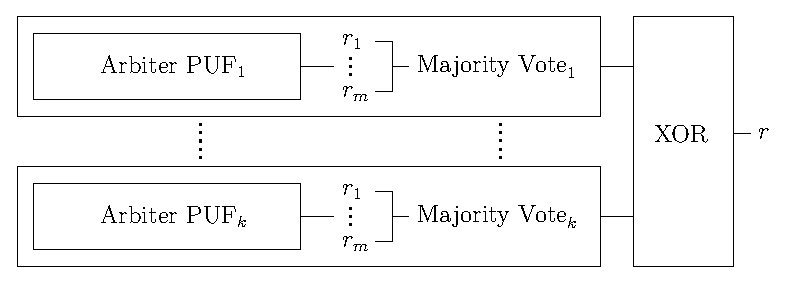
\includegraphics[width=1.00\textwidth]{images/majority_xor_arbiter_v2.eps}
% \noindent\includegraphics[width=1.00\textwidth, height=3cm, draft]{example-image-a}
\caption[Majority \acs{XOR} \apuf]{\mxpuf}
\label{fig:majorityxorarbiter}
\end{figure}

%========================================

\section{Combiner Functions}
\label{sec:combinerfunctions}
% \section{Majority based bent arbiter PUFs}
% \label{sec:majoritybentarbiter}

Beside the \ac{XOR} function other Boolean functions could be used to combine multiple \apuf.
In addition to being a Boolean function it is important that the function obfuscates the single responses of the \apufs. 
Otherwise, the \apufs are directly vulnerable to modeling attacks on \apufs.
% [https://en.wikipedia.org/wiki/Avalanche_effect#Strict_avalanche_criterion]
% Bent functions are a type of Boolean function which meets these requirements for example. 
% They are highly non-linear which is desired in this case as the \apuf itself is linear and can therefore badly resist machine learning attacks.
%This prevents predictions about the input based on an analysis of the output of the function.

Bent functions are one example for Boolean functions, which can be used instead of the \ac{XOR} function \cite{Adams1990Thedesign,Forre1990Thedefinition,Seberry1993Highlycriterion}.
%old: They are highly non-linear, which is desired in this case since \apufs can be represented by a linear threshold function that can be attacked successfully, as described in Sec.\ \ref{sec:attacksonarbiter}.
They are highly non-linear, which is desired in the case of \apufs, since they can be represented by a linear threshold functions.
Attacks mentioned in Sec.\ \ref{sec:attacksonarbiter} are able to successfully attack these linear threshold functions.
The non-linearity increases the complexity of attacks, as described in Sec.\ \ref{sec:xorarbiterpufs}. %+
Beyond that Bent functions fulfill the strict avalanche criterion \cite{Feistel1973Cryptographyprivacy}.
The strict avalanche criterion means if any number of input bits is flipped the output bit flips with a likelihood of $50\ \%$.

How these attributes of Bent functions can help to prevent successful attacks and analysis of the underlying \apufs has to be examined.
This thesis is focused only on the \ac{XOR} function used as combiner function and will not consider other possible combiner functions further.

%========================================
% source?!
